%
% File: chap01.tex
% Author: Liam O'Shea
% Description: Introduction chapter where the boxing goes.
%
\let\textcircled=\pgftextcircled
\chapter{Specification and Design}

\initial{I}n this chapter we will analyse a variety of different techniques for their suitability for this project. Each individual stage will be discussed, collection of data, dimensionality reduction, punch segmentation and punch classification with the goal of developing a pipeline to implement.


%=======
\section{Scope of Project}
\label{sec:sec01}
\textcolor{red}{
The `orthodox' stance will be used, meaning only those who are right handed will be able to use this implementation.
Cannot deal with movement while punch is being thrown.
Need to be a set distance from the Kinect.}

\section{Dimensionality}
\paragraph{Curse of Dimensionality}
The curse of dimensionality, first discussed by Richard E Bellman in his book Dynamic Programming\cite{dynprog} is the term for a set of problems that occur when using high dimensionality data. As dimensionality increases as does the search space, resulting in the available data become sparse. In order to obtain accurate, reliable and statistically sound results the total amount of data required can grow exponentially in relation to the dimensionality. Likewise the organisation and searching of non-reduced data becomes difficult, with space and search time dependent on data volume. Searching and organising data also relies on the ability to group instances into groups that share similar characteristics, unfortunately if the data appears to be dissimilar due to sparseness it can prevent grouping strategies.

Algorithms that can successfully deal with high dimensionality data typically will have high time complexity and {\bf will not always} produce more accurate results than algorithms that work on the lower dimensionality data. Therefore it is sensible to look at some dimensionality reduction techniques which {\bf might}produce better results.

Furthermore since the long-term goal is to give feedback with live data, speed is of the essence. Therefore dimensionality reduction is an important component required to decrease the processing time on any input.

\subsection{Dimensionality Reduction}
Dimensionality Reduction is the process of reducing the number of variables under consideration for any given problem. For example each frame from the Kinect is represented by 80 data points, 60 of which are the x,y,z co-ordinates of the 20 skeleton joints. Considering the Kinect is capable of 30 FPS that is $1800$ data points per second of movement. With long sequences of recordings this could become a huge amount of data to process, most of which could be represented in a reduced dimensionality.

\subsection{Principal Component Analysis (PCA)}
\label{subsec:subsec01}
Principal Component Analysis is a statistical procedure that transforms a set of observations of potentially correlated variables into a set of linearly uncorrelated variables called principal components. The number of principal components should always be less than or equal to the number of original values with the first principal component having the largest possible variance. Each following component will attempt to represent as much variance in the data as possible. In my case I will be looking to reduce my 60 data points per frame into a low dimensionality set that will help me to uniquely identify punches.

The principal components

\begin{figure}[h]
    \centering
    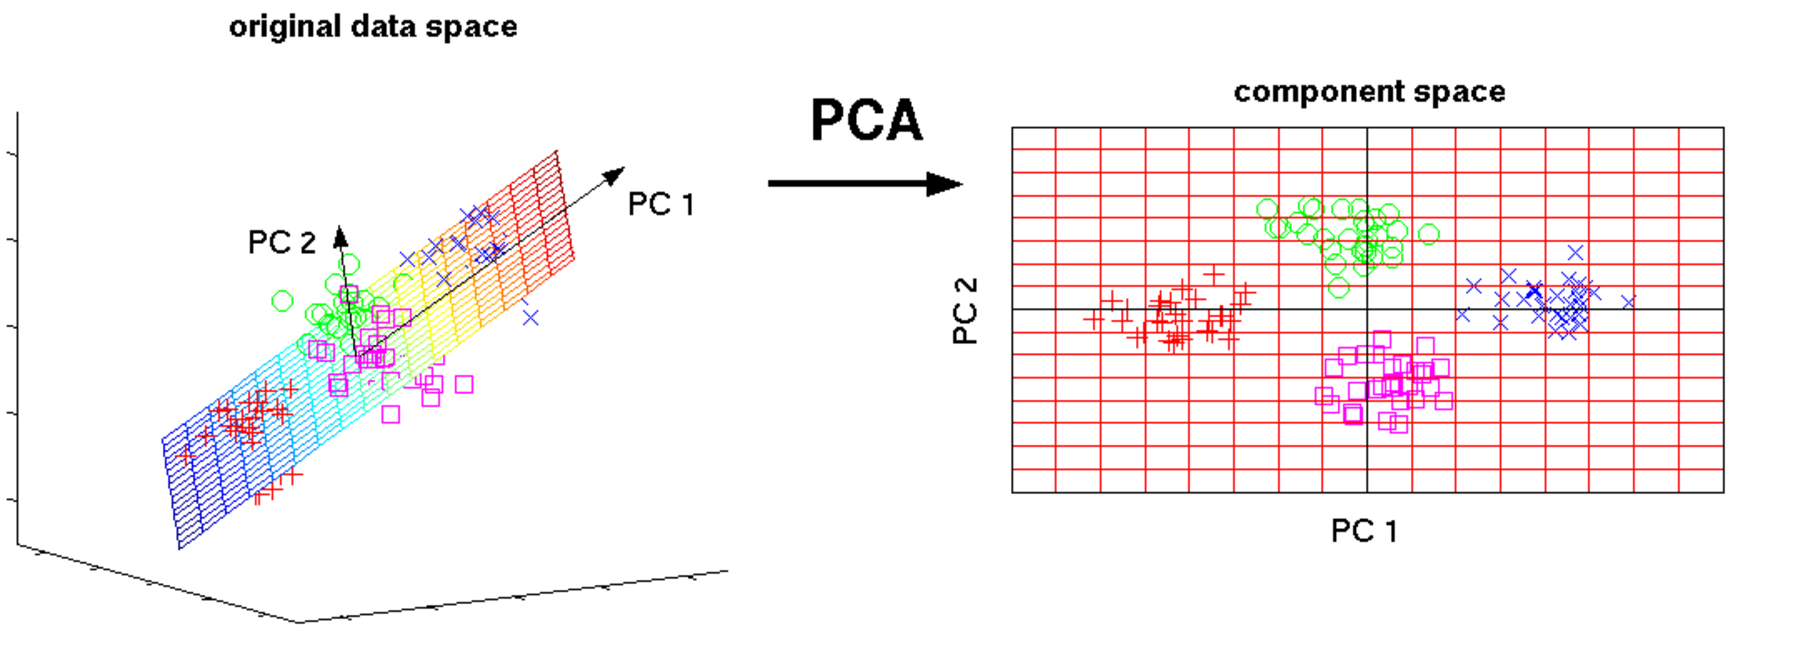
\includegraphics[height=0.25\textheight]{fig03/PCA.pdf}
    \mycaption[PCA Example]{Example of PCA reduction}
    \label{fig:kinect}
\end{figure}

\section{Manifold Learning}
Manifold learning is a Non-Linear Dimensionality Reduction process that transforms high dimensionality data that typically requires multiple dimension to represent it which is difficult to interpret. To simplify the data it is possible to assume that the date lies on an embedded non-linear manifold within the high-dimensionality space. Assuming the manifold has low enough dimensions it can then be visualised in this lower-dimensionality space.

\subsection{Markov Chains}
Markov chains are a series of `states' which have a probability for each transition and are used to model real world events.

\begin{figure}[h]
    \centering
    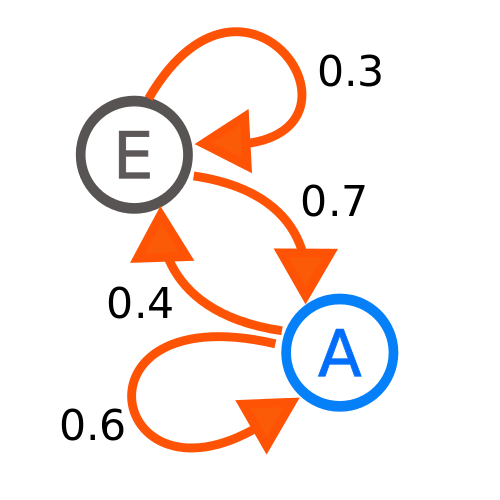
\includegraphics[height=0.25\textheight]{fig03/markov}
    \mycaption[Kinect Device]{Kinect Device.}
    \label{fig:kinect}
\end{figure}

\subsection{Diffusion Maps}
Diffusion maps are a non-linear and relatively new technique developed in $2006$ by Ronald R. Coifman and Stephane Lafon.\cite{Coifman2006} The aim of a diffusion map is to provide a framework for finding meaningful geometric descriptions of data sets. Diffusion maps are capable of turning high dimensionality data into low dimensional structure. Unlike other dimensionality reduction techniques like PCA, diffusion maps attempt to discover the underlying manifold, a lower dimensional constrained surface containing the data. Diffusion maps are based on defining a Markov chain on the graph of the data. By performing this for a set number of time steps a measure for the proximity of data points is obtained, which is used to define a diffusion distance. Pairwise diffusion distance are retained as well as possible in the dimensionally reduced data.

\begin{figure}[h]
\centering
\begin{minipage}{7.0cm}
    \centering
    \subtop[]{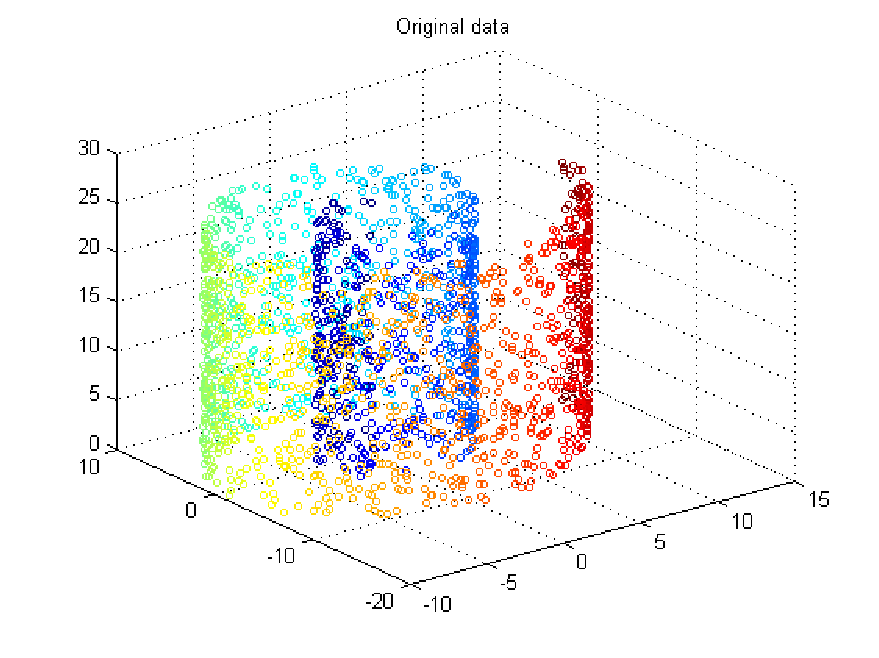
\includegraphics[height=0.25\textheight]{fig03/diffmap1.pdf}}
    \label{fig:1}
\end{minipage}
\vspace{2.0cm}
\begin{minipage}{7.0cm}
    \centering
    \subtop[]{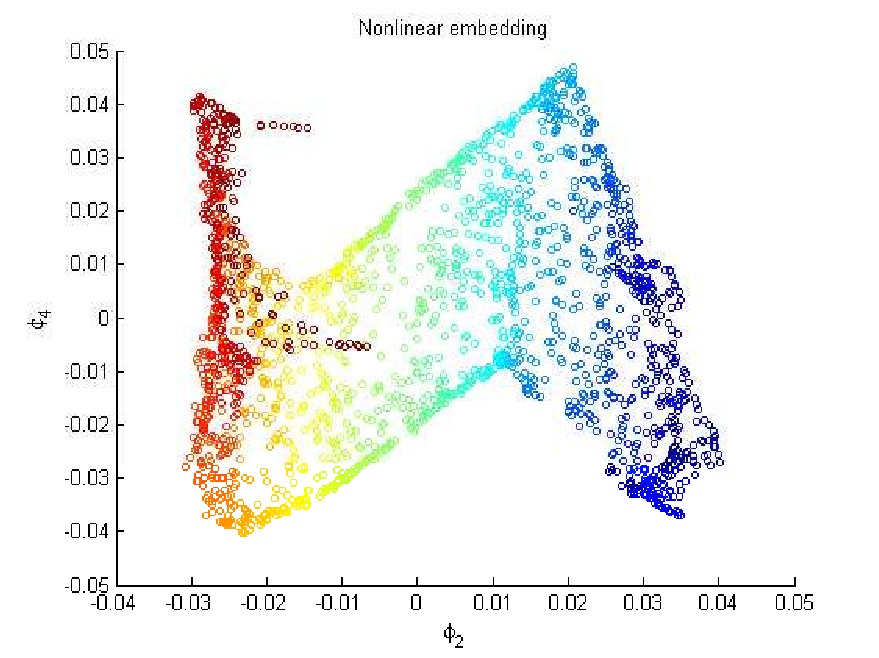
\includegraphics[height=0.25\textheight]{fig03/balls.pdf}}
    \label{fig:2}
\end{minipage}
\mycaption[ALLData] {(a) Original example data 
(b) Non-linear embedding}
\end{figure}


\subsection{Locally Linear Embedding (LLE)}
In LLE a data manifold is constructed by finding a set of the nearest neighbours for each point\cite{Roweis2000}. Together they are used to compute a set of weights that describes each point as a linear combination of its neighbours. Finally, it uses an eigenvector-based technique to find the low-dimensional embedding of points, such that each point is still described with the same linear combination of its neighbours. Furthermore, the preservation of local properties allows for successful embedding of non convex manifolds.
{\bf LLE tends to handle non-uniform sample densities poorly because there is no fixed unit to prevent the weights from drifting as various regions differ in sample densities.}

\subsection{Laplacian Eigenmaps}
Laplacian Eigenmaps find a low-dimensional data representation by preserving local properties of the manifold.\cite{Belkin2003} Similar to LLE, a graph is built from neighbourhood information, with the distance between a point and it's K nearest neighbour is minimised. A weighting system is used such that in the low-dimensionality space the distance from a point to it's nearest neighbour is more significant to the cost function than other nearby points. {\bf put simply the closer a neighbour is to the selected data point the heavier its weighting.} The goal overall is to minimise the cost function based on the graph information to ensure that points close together in the high dimensionality data remain so after the reduction, preserving local distances. 


\subsection{Local Tangent Space Alignment (LTSA)}
LTSA is based on the intuition that when a manifold is correctly unfolded, all of the tangent hyperplanes to the manifold will become aligned.\cite{Zhang2003} In other words there will exist a linear mapping from high dimensionality data to a local tangent space which will have a linear mapping to a low-dimensionality data point. It begins by computing the k-nearest neighbours of every point. It computes the tangent space at every point by computing the d-first principal components in each local neighbourhood. It then optimizes to find an embedding that aligns the tangent spaces.


\subsection{Curvilinear Component Analysis (CCA)}
CCA is an learning algorithm that starts with larger distances before iterating to smaller ones.\cite{Demartines1997} It looks to output a configuration of points that preserves the original distances as much as possible while focusing on the smaller distances.

The large distance information will be overwritten by the smaller distance information unless a conflict occurs. The stress function of CCA is related to the sum of Bregman divergences which aim to generalise squared euclidean distances so they all share the same properties. If compromises between the larger and smaller distance information but be made the stress function determines this.

\subsection{Comparison Methods}
Each comparison method was evaluated on it's ability to produce useful, smooth and sinusoidal output to aid automatic segmentation. Automatic segmentation is a crucial step in the project since on a larger scale much greater data sets will need to be used and collated from multiple sources. If these can be processed and automatically segmented this will remove any manual work required and make this a truly useful system.

\begin{figure}[h]
    \centering
    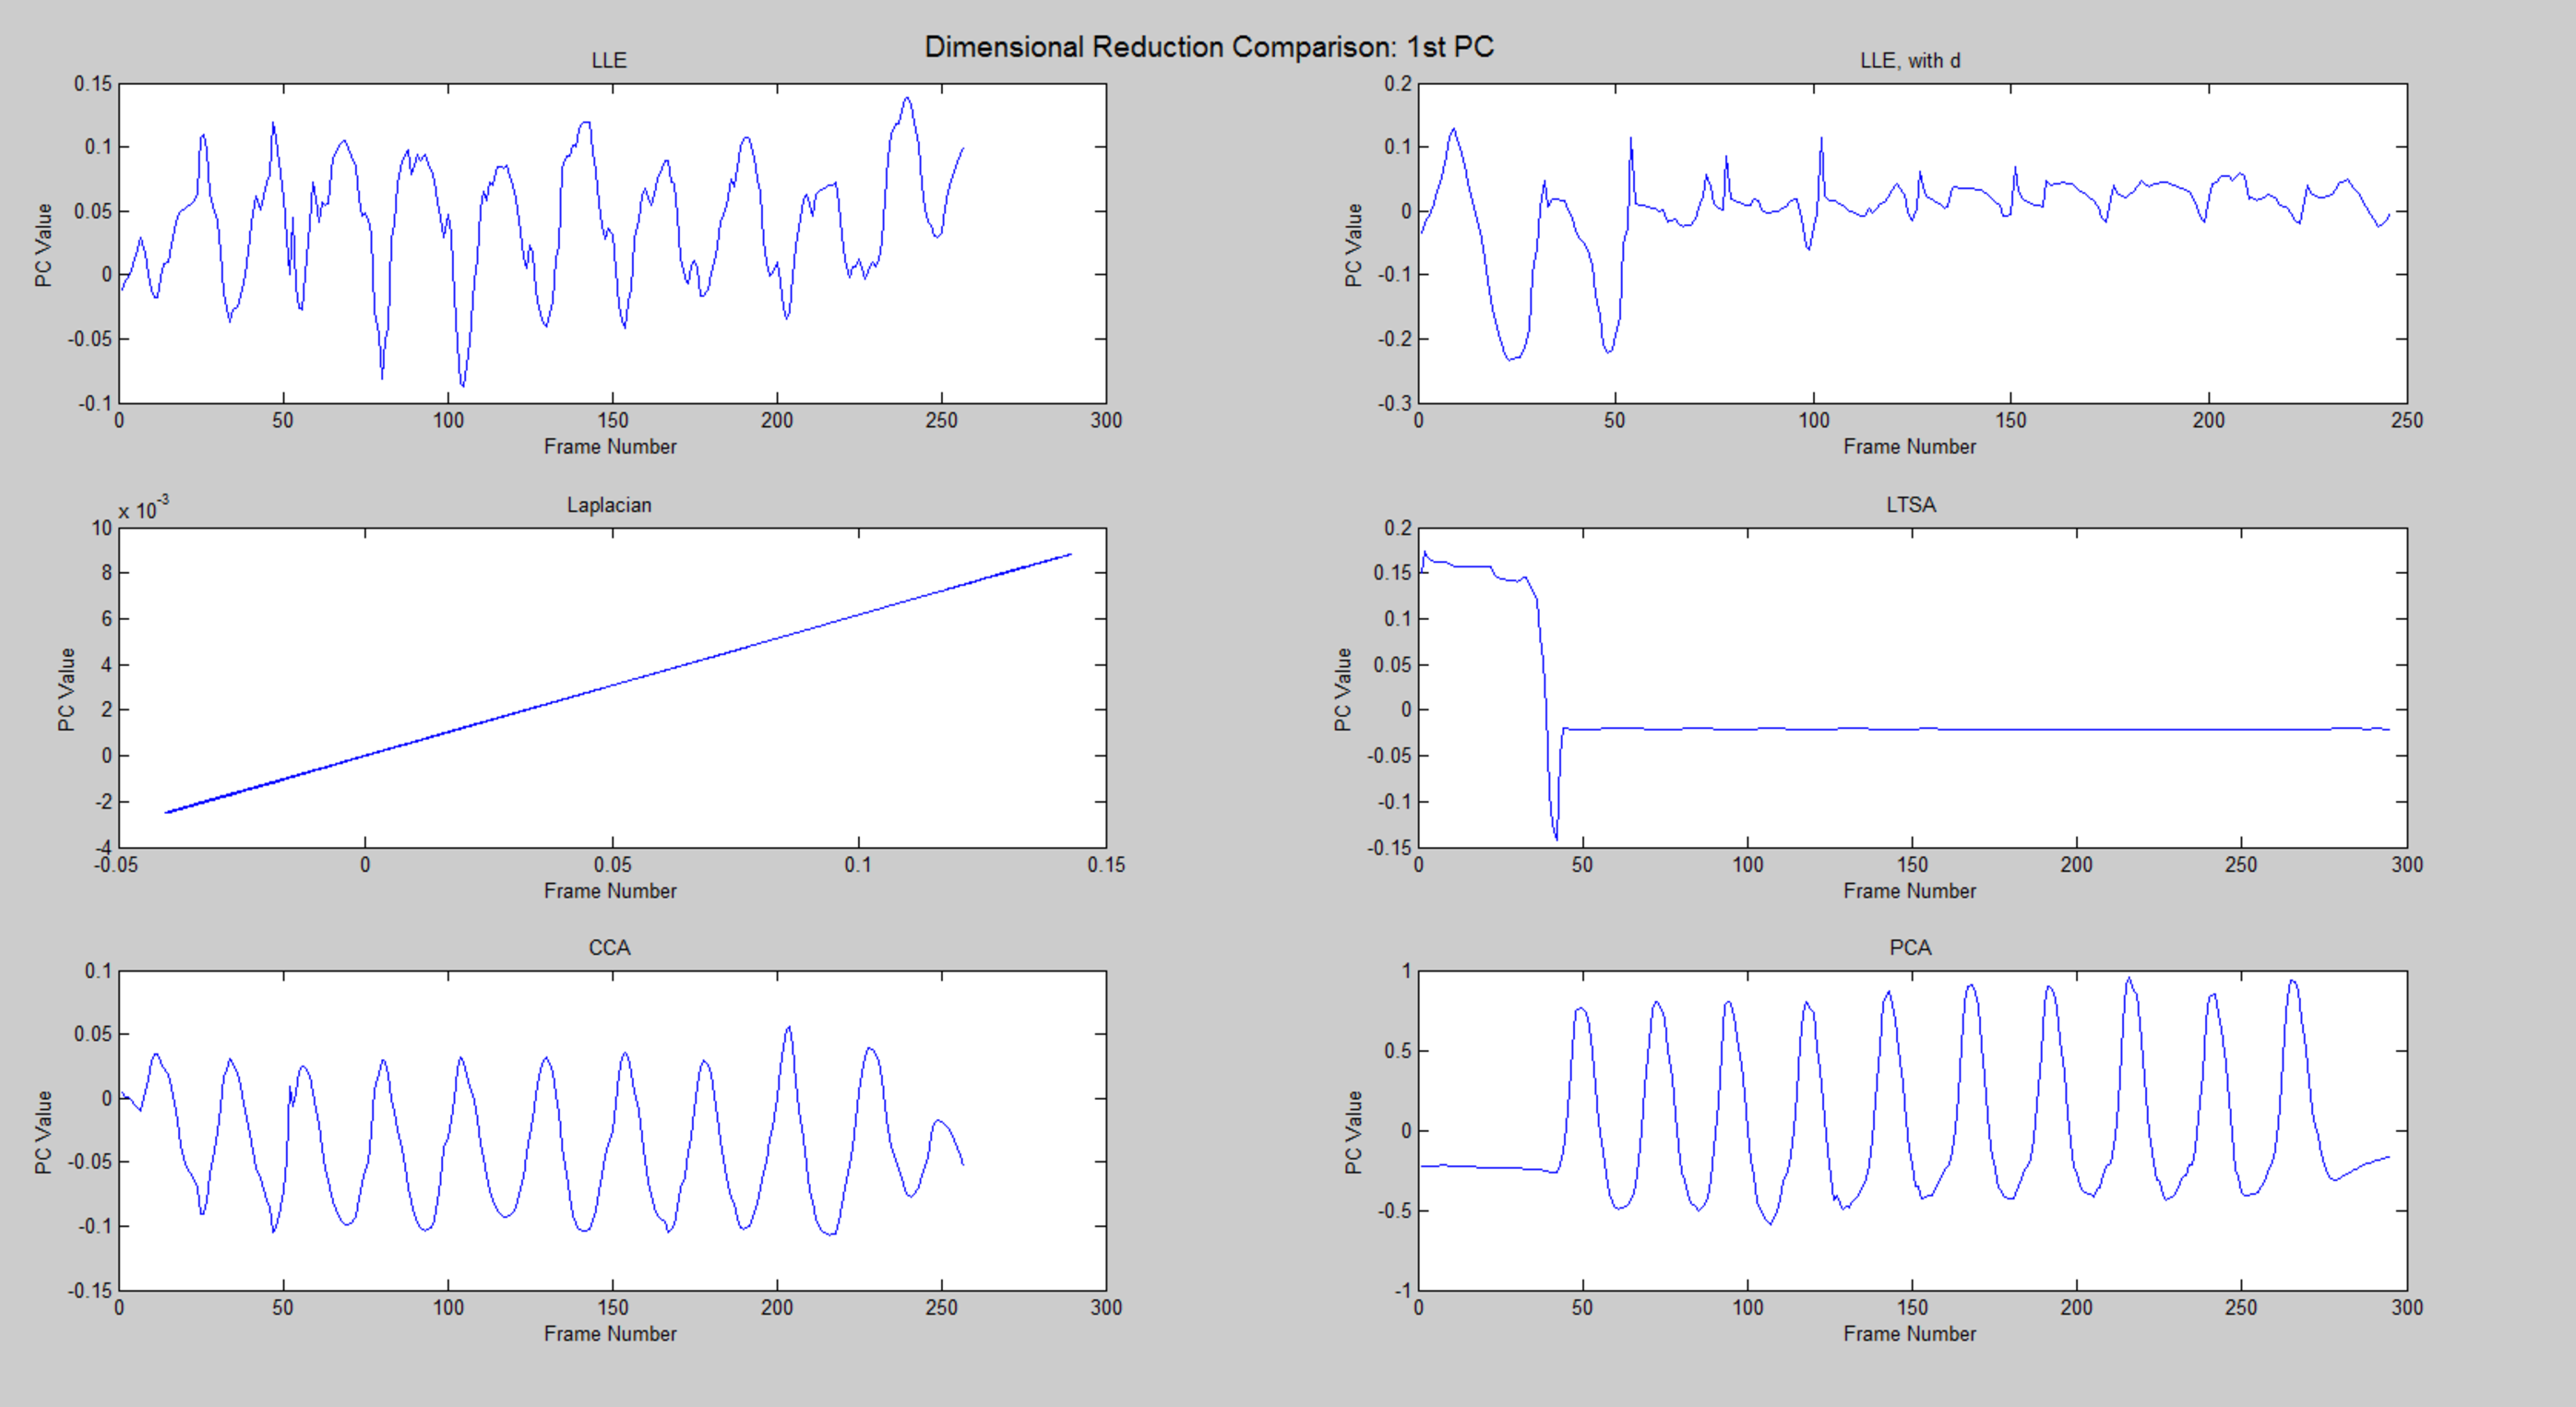
\includegraphics[height=0.25\textheight]{fig03/drcomp.pdf}
    \mycaption[Kinect Device]{1st PCA comparison}
    \label{fig:drcomp}
\end{figure}
\begin{figure}[h]
    \centering
    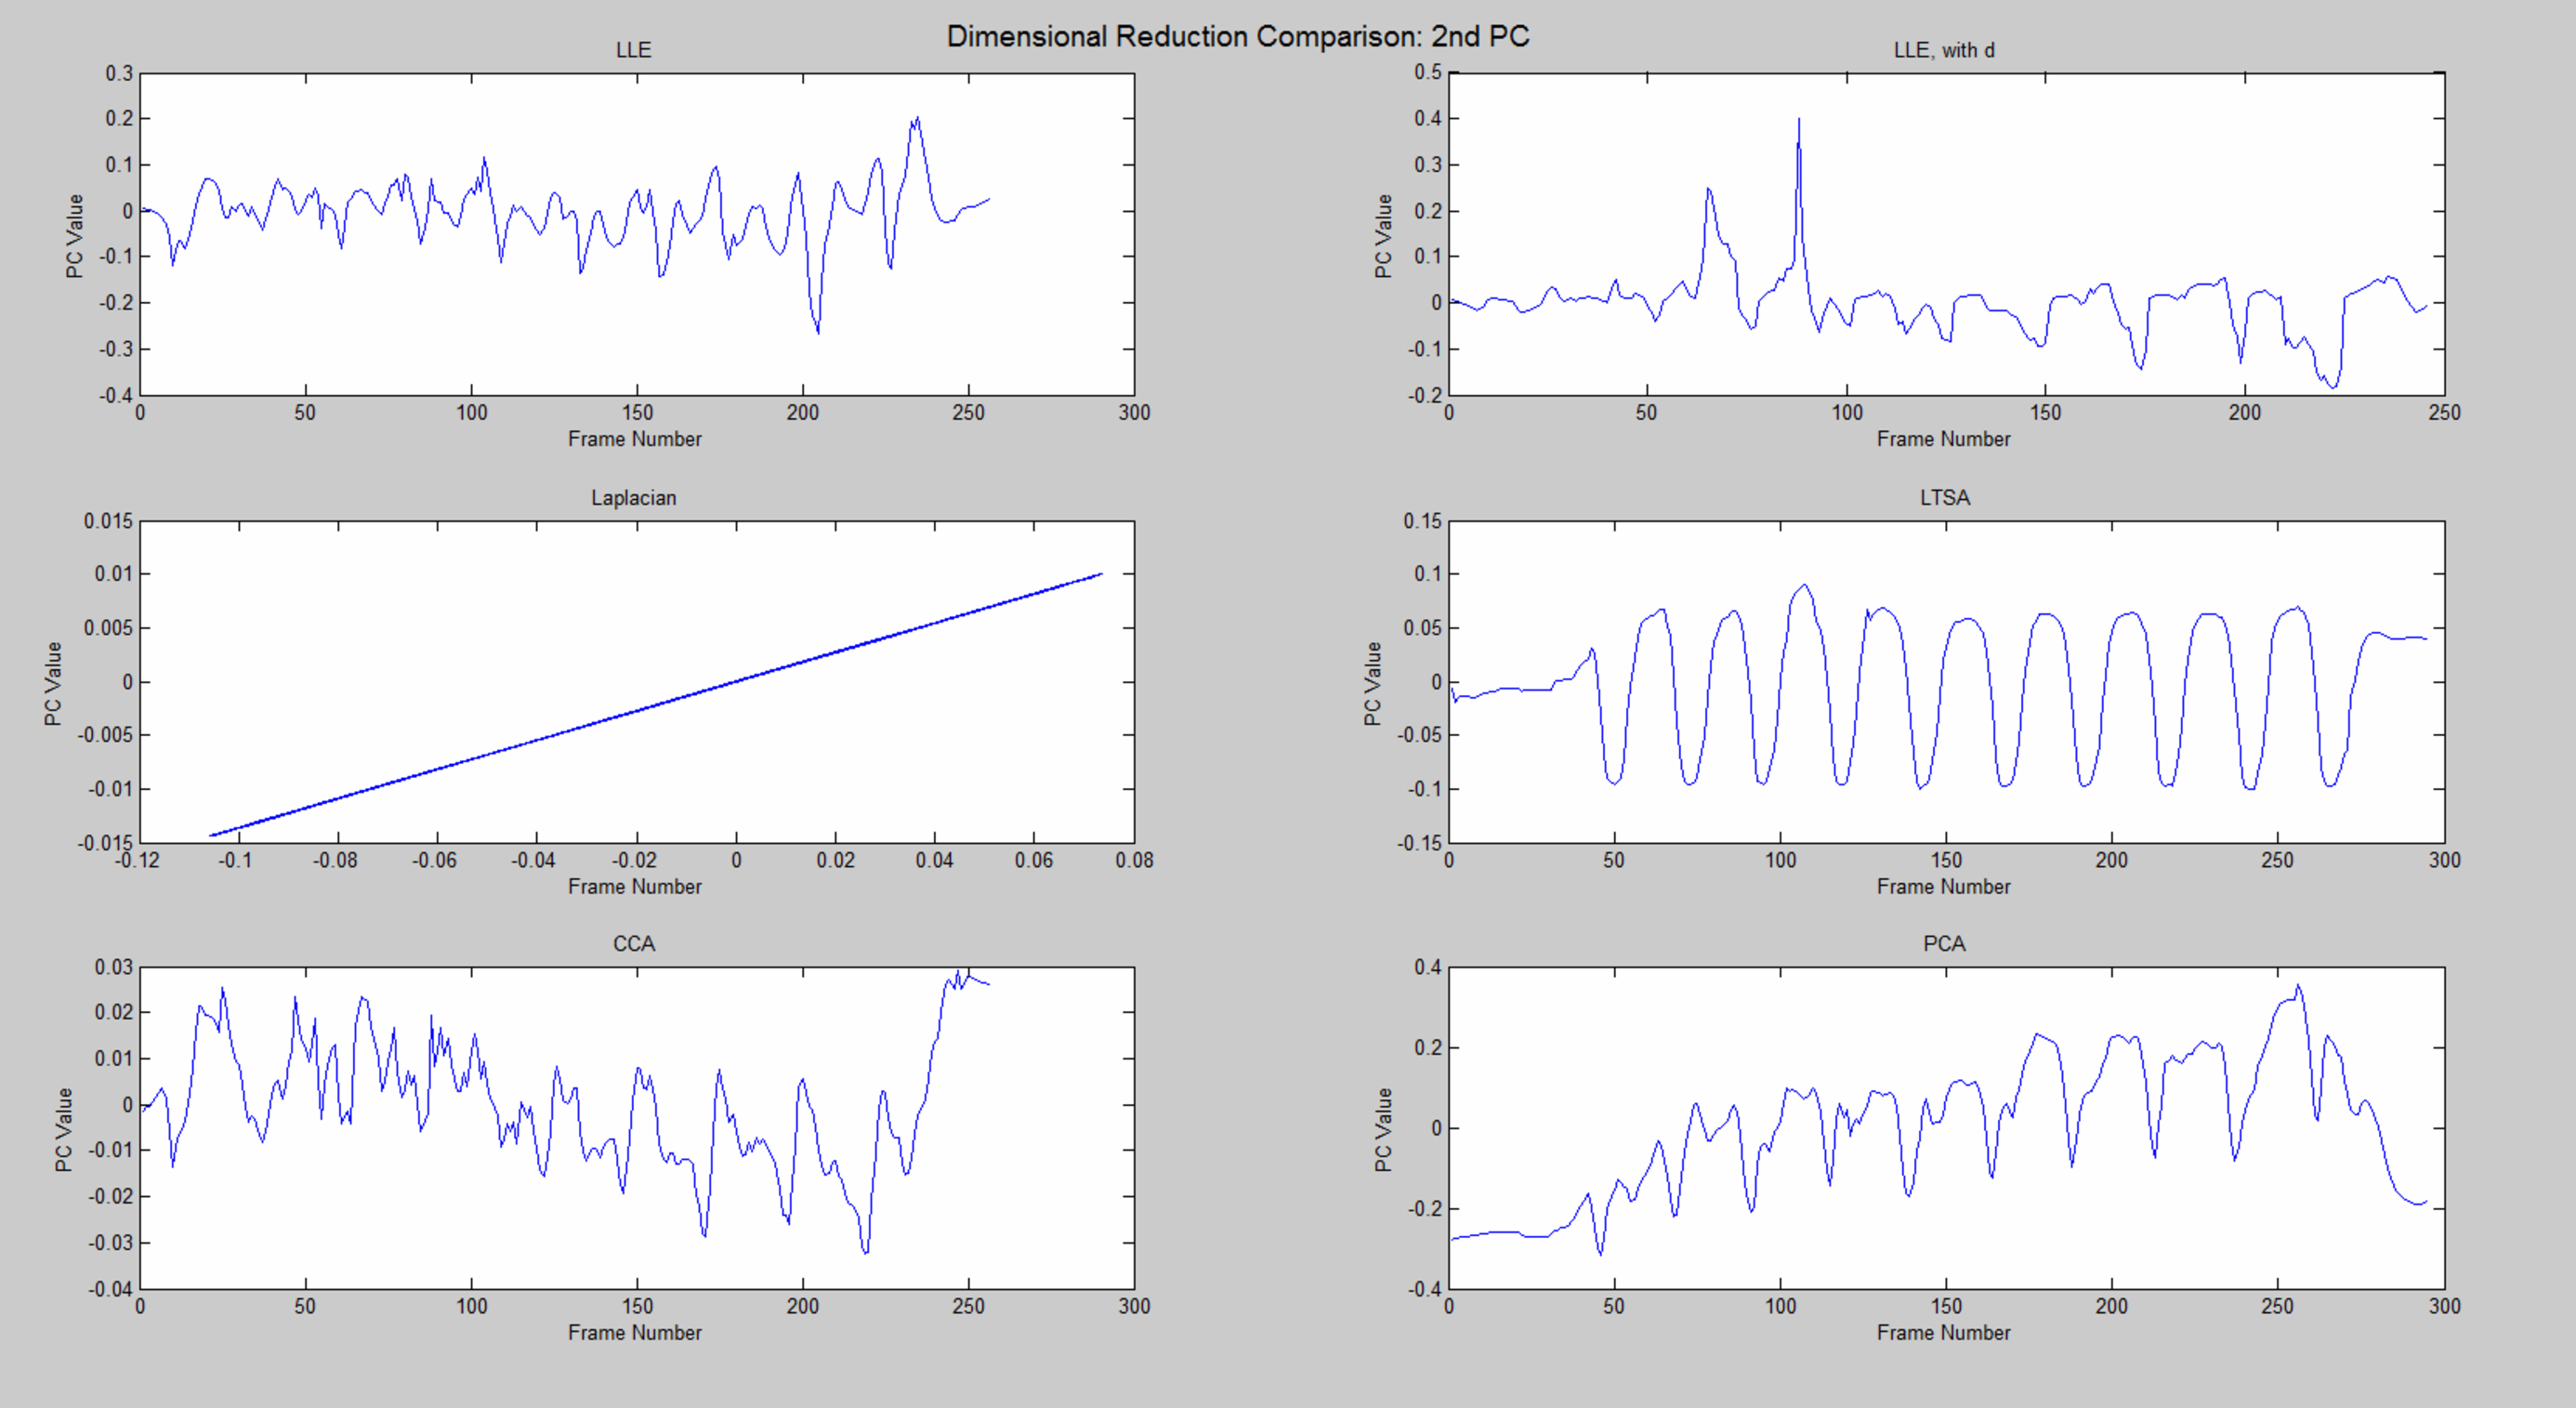
\includegraphics[height=0.25\textheight]{fig03/drcomp2.pdf}
    \mycaption[Kinect Device]{1st PCA comparison}
    \label{fig:drcomp}
\end{figure}

We can see from the first principal component plotted from multiple dimensionality reduction method that PCA does in fact give the most useful results, followed closely by CCA. If we then look at the second principal components we can see that PCA performs second to LTSA but since LTSA performs poorly for the first component it makes PCA the obvious choice.


\section{Segmentation Methods}

\subsection{Dynamic Time Warping (DTW)}
Dynamic time warping compares two temporal sequences, often which vary in time or speed and tries to calculate an optimal match. The two sequences are aligned and a similarity score is produced. This technique can be used on any data that can be represented in a linear fashion and has been successfully applied to fields such as signature recognition, voice recognition, partial shape matching and gait analysis. For example in gait analysis, similarities could be detected in the walking pattern of two people even though their speed and acceleration may be difference. 

After using dynamic time warping I found that there was not enough difference between the various punch signals to give me an effective way at segmentation. Comparing jabs to other jabs yielded similarity values from $0 - 1.589$ with an average difference of $0.499$, comparing jabs to crosses yielded similarity values from $0-2.113$ with the average $0.716$. Therefore there was not enough of a consistent difference score to be able to classify they type of punch using this method.


\begin{figure}[h]
    \centering
    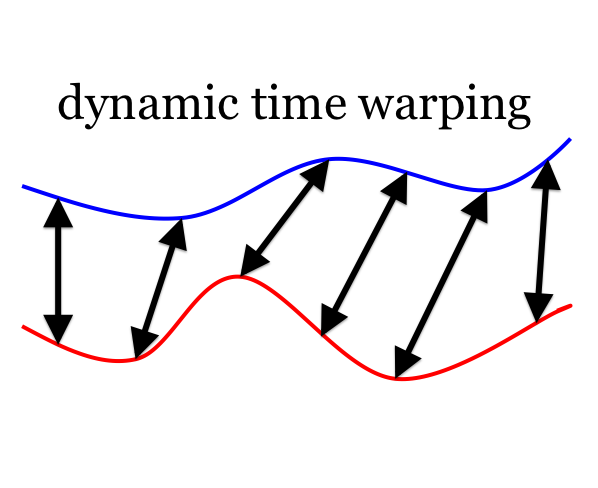
\includegraphics[height=0.25\textheight]{fig03/dtw}
    \mycaption[Kinect Device]{Dynamic time Warping}
    \label{fig:kinect}
\end{figure}


\subsection{Fourier Transformation}
The FT is a mathematical transformation that transforms signals from the spatial domain (normal image space) into the frequency domain. It allows a signal to be split in a phase and magnitude spectrum.Since my punches are a continuous periodic function over time, the Fourier transformation can be simplified to a set of complex amplitudes know as Fourier Series Coefficients. These represent the frequency domain of the original signal and can be used to recreate the signal if required. I investigated the possibility of running a fast Fourier transform (FFT) on the raw data as well as each segmented punch that was later obtained from using PCA and my own segmentation algorithm. The range for the coefficients was $0 - (63.030 - 0i)$ with a spread across all of the different types of punches. 
Unfortunately this meant the coefficients obtained in both cases proved to be a poor differentiator between punches due to the coefficients being so variable even within the same punch types.

\subsection{Punch Segmentation Algorithm}
After failing to find a way to automatically segment punches using existing methods It became apparent that a custom algorithm will be needed for this task, which can be broken down into several steps.

\begin{enumerate}[noitemsep]
  \item Perform PCA on raw data.
  \item Smooth the principal coefficients. \textcolor{red}{Rember 1st pc}
  \item Find the local maxima and minima for the punch sequence.
  \item Remove erroneous Minima\/Maxima using heuristic rules.
  \item Take a number of evenly spaced samples from between two maximum points, the length of one punch.
  \item Fetch all PCA components that correspond to the time the samples were taken.
  \item Train classifier on new data.
\end{enumerate}

Each frame representing 20 joint positions is reduced from 60 dimensions to 3 principal components per frame. Next the principal components are smoothed to remove any {\bf wrong minima/maxima} which would prevent the automated segmentation of punches. All remaining maxima are then passed through a set of heuristic rules that checks the location of a maxima point relative to it's neighbourhood points to determine if it is legitimate. The simplest form of this is using the Pythagorean theorem to calculate the distance between a maxima and it's neighbours, if the distance is too small it is clear that one of the points is erroneous and that only one of these will be necessary for segmentation. Likewise if a neighbour is too far away it becomes obvious that one of the maxima is incorrect and needs to be removed.\textcolor{red}{image showing points really far down compared to baseline} Thresholding is also used for each punch, with all maxima below a certain threshold removed since the cyclical signature of the punch guarantees the end of the punch will be approximately close to the end of the last punch.

Once the data has been successfully segmented into individual punches we can begin to extract features that can be used to train a classifier. Between 12 and 15 evenly spaced samples are taken for each individual punch, depending on the classifier to be used later. Each sample corresponds to a point in time which is used to extract the 3 principal coefficients for each point which results in a $36 - 45$ features for each punch.

Once all the different punch sequences are sampled for each type of punch we can use this data to train a classifier. A multi-class SVM, decision tree, Random Forest and neural network were tested. .............

Results


\section{Classification Methods}

\subsection{Support Vector Machines}
A Support Vector Machine is a kernel-based method that is effective for highly dimensional datasets. The SVM uses a kernel to calculate the scalar product of two feature vectors in a high dimensional feature space. The decision function uses the hyper-planes, defined by the Support  vectors,  to  classify  the  data.  Only  significant  samples  are  taken  for  use  as support vectors so that a high variance will make less of a different to the accuracy of the model. \textcolor{red}{This is well suited to a recognition task as the same punches will be thrown slightly differently.}

\begin{figure}[h]
    \centering
    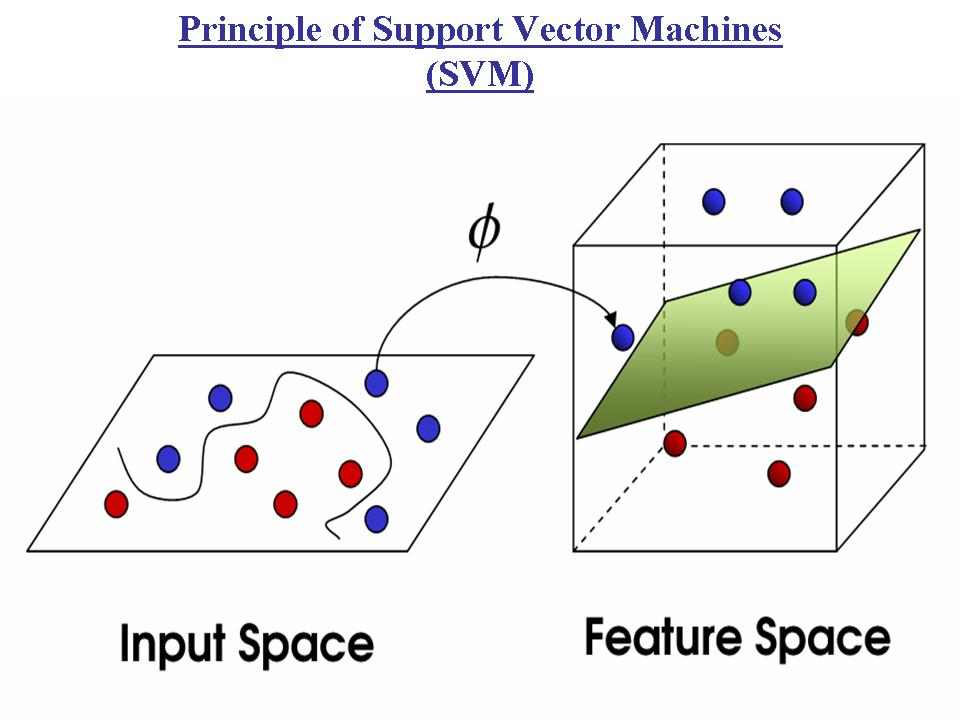
\includegraphics[height=0.25\textheight]{fig03/svm}
    \mycaption[Kinect Device]{Kinect Device.}
    \label{fig:kinect}
\end{figure}

\subsection{Neural Networks}
Neural networks are models based on the parallel processing of information similar to that of the brain. A NN can be configured for different applications such as clustering, pattern recognition, Dynamic Time series and curve fitting. They are able to derive meaning from complex data that human beings would be unable to notice and that other techniques will fail on. Crucially the networks are capable of approximating non-linear functions \textbf{unlike DTW. Neural networks learn by examples in the form of training data and are adaptive based on a system of weightings calculated by \% error. Other characteristics are their ability to self organise and the ability to work in real-time if sufficient parallelism is supported.}

\subsection{Decision Trees \& Random Forest}
A predictive tree like model which maps observations about an object to reach a conclusion about its target value. In this model the `leaves' represent class labels while the branches themselves represent conjunctions of features that will lead to the class labels. Put simply each condition in an internal node while each outcome is an external node. Information gain is the difference between the initial entropy and the new entropy after following a branch along the decision tree. Since the goal of any machine learning technique is to achieve a low value of entropy to make accurate predictions, the decision tree is constructed such that each branch has the maximum possible information gain. The data is split by each feature that has the maximum information gain recursively for each branch.

Bagging is a method of assigning a measure of accuracy to sample estimates. We sample from an approximating distribution and try to approximately calculate the
properties of the estimator based on this. We measure a statistic from a sample of the population and then use this to say something about the whole population. For example, we might say that for our set of data a subset is used to determine a class. If any sample in the entire population follows the same tree rules then it will be labelled as in that class. We have used bootstrapped samples in our classifiers as they have been constructed using random sampling with replacement. 
This method is designed to improve the accuracy of machine learning algorithms, helping to reduce variance and hence over fitting. 

Random forest is an averaging algorithm which produces a diverse set of classifiers by introducing randomness in the classifier construction. Each tree is built from a bootstrapped sample from the training set. During construction the node splits are chosen based on the best split among a random subset of features, not the best split among all the features. Due to the randomness of this algorithm we expect it to have a slight bias compared to other decision tree
models, however due to the averaging we expect a lower variance.

These Ensemble methods combine the predictions of multiple trees to come to a consensus.



\textcolor{red}{Bootstrapping because our data is from an independent and identically distributed
population.?}
\textcolor{red}{Why did RF perform worse?}
 


\begin{figure}[h]
    \centering
    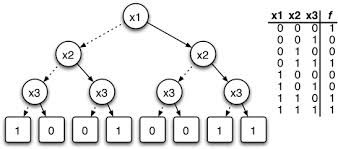
\includegraphics[height=0.25\textheight]{fig03/dtree}
    \mycaption[Kinect Device]{Kinect Device.}
    \label{fig:kinect}
\end{figure}


%=========================================================
\section{Punch Quality Algorithm}
I will be measuring quality in reference to a `ground truth' produced by a local professional. My aim is to create rules that are capable of detecting basic mistakes and provide feedback. I will start by targeting the characteristics as mentioned in the earlier background chapter, for example 
throwing a jab with the elbow sticking out instead of tucked is a classic beginners mistake.

